\svnid{$Id: funktionen.tex 108 2012-05-12 18:44:01Z dgens001 $}
\chapter{Abläufe und Funktionen}

\textit{Dieses Kapitel bietet einen Einblick in das Zusammenspiel der Prozesse und Abläufe des Spiels.
Anwendungsfälle der Interaktionen mit dem System, dabei wichtige Anwendungsfunktionen und die jeweiligen 
Akteure sollen einen klaren Umriss des später implementierten Spiels geben.}

\section{Menümodus}
Nach dem Start der Anwendung findet sich der \gls{Spieler} im Menümodus. Von dort aus kann er die Funktionen
des Hauptmenüs erreichen und in andere Menüsichten wechseln. Unter Optionen könnte eine Reihe von 
Einstellungen getroffen werden, zumindest soll hier die Ingamesteuerung konfigurierbar sein. Später könnten
auch zusätzliche Sound- oder Videoeinstellungen hier vorgenommen werden. Die Funktion \textit{Spiel beenden}
beendet die Applikation.

\begin{figure}[htb]
	\begin{center} 
		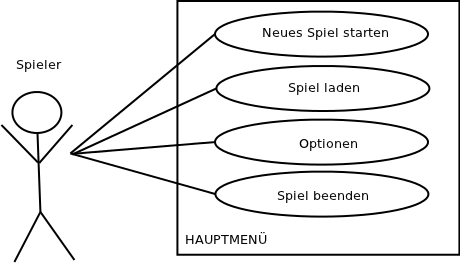
\includegraphics[width=100mm, height=60mm]
                  {kapitel/funktionen/Hauptmenue.png}
	\end{center}
	\caption{Übersicht der Hauptmenü-Funktionen}
	\label{fig:hauptmenue_funktionen}
\end{figure}

Neben dem Menümodus mit seinen verschiedenen Sichten gibt es den Ingamemodus, in dem das eigentliche Spiel
abläuft. Die Funktionen \textit{Spiel laden} und \textit{Neues Spiel starten} wechseln vom Menü- in den
Ingamemodus. Startet man ein neues Spiel, muss zunächst ein \gls{Campus} geladen werden. Hierzu wählt man 
aus einer zuvor erstellten Liste eine Campusdatei aus. Die \gls{Welt} wird anhand dieser Datei automatisch 
erstellt. Bestätigt der Spieler seine Campuswahl, wechselt das System automatisch in den Ingamemodus und
startet auf dem gewählten Campus.

\paragraph{UseCase: Neues Spiel starten}
\begin{center}
	\begin{tabular}{|r l|}
	  \hline
	  \textbf{Titel}: & Neues Spiel starten \\
	  \textbf{Akteur}: & \gls{Spieler} \\
	  \textbf{Fachlicher Auslöser}: & \gls{Spieler} hat \textit{Neues Spiel starten} gewählt \\
	  \textbf{Vorbedingung}: & Das System hat Zugriff auf mindestens eine Campusdatei \\
	  \hline
	  \textbf{Standardablauf}:
		& 1. Spieler: Wählt einen Campus aus \\
		& 2. Spieler: Bestätigt Campuswahl \\
		& 3. System: Liest die Campusdatei ein \\
	  \textbf{Abbruch}:
		& 1a. Spieler: Wählt \textit{Zurück} \\
		& 2a. System: Wechselt ins Hauptmenü \\
	  \hline
	  \textbf{Nachbedingung}: & System geht in Zustand \gls{Ingame} oder Hauptmenü \\
	  \textbf{NF-Anf}.: & Ladezeit $<$ 30 Sekunden \\
	  \textbf{Parameter}: & Campusdatei \\
	  \textbf{Nutzungshäufigkeit}: & bei jedem neuen Spiel \\
	  \hline
	\end{tabular}
\end{center}
\newpage
\section{Ingamemodus}
Der Ingamemodus ist der wichtigste Zustand der Applikation. Hier bieten sich dem Spieler alle Möglichkeiten,
er kann den Campus erkunden, Gegenstände aufnehmen oder ablegen, mit NPCs reden, neue Räume betreten usw.
Im Wesentlichen lassen sich die Funktionen wie in Abb. \ref{fig:ingame_funktionen} dargestellt zusammenfassen.

\begin{figure}[htb]
	\begin{center} 
		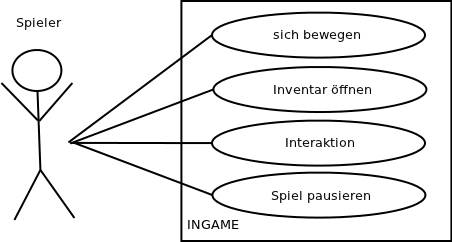
\includegraphics[width=100mm, height=50mm]
                  {kapitel/funktionen/InGame.png}
	\end{center}
	\caption{Übersicht der Ingame-Funktionen}
	\label{fig:ingame_funktionen}
\end{figure}

\subsection{Charakterbewegung}
Der \gls{Spieler} kann sich grundsätzlich über entsprechende Tasten von Feld
zu Feld bewegen oder seine Sicht innerhalb eines Feldes steuern. Dabei behält der
\gls {Spieler} bei seitlichen Bewegungen über Felder stets seine Blickrichtung bei (sogenanntes Strafing).
Die Blickrichtung kann er ändern, indem er sich auf einem Feld nach Links oder Rechts dreht.
Grundsätzlich gibt es nur vier Blickrichtungen auf jedem Feld, die mit Nord, Süd, Ost und
West bezeichnet werden. Bei Bewegung nach vorn oder hinten behält der Spieler ebenfalls seine Blickrichtung
bei (die Ansicht wechselt also nicht um $180 ^{\circ}$ wenn der Spieler rückwärts gehen möchte). 

\subsubsection{UseCase: Charakterbewegung}
\begin{center}
	\begin{tabular}{|r l|}
	  \hline
	  \textbf{Titel}: & Charakterbewegung\\
	  \textbf{Akteur}: & Spieler \\
	  \textbf{Fachlicher Auslöser}: & Spieler wählt Bewegungsrichtung \\
	  \textbf{Vorbedingungen}: & Spieler ist Ingame \\
	  \hline
	  \textbf{Laufen}:
		& 1. Spieler: Möchte nach vorn oder hinten laufen \\
		& 2. System: Versetzt den Spieler auf das Feld seiner Wahl \\
		& 3. System: Wechselt die Ansicht zum neuen Feld \\
	  \textbf{Strafen}:
		& 1. Spieler: Möchte nach rechts oder links strafen \\
		& 2. System: Versetzt den Spieler auf das Feld seiner Wahl \\
		& 3. System: Wechselt die Ansicht zum neuen Feld \\
	  \textbf{Drehen}:
		& 1. Spieler: Möchte Blickrichtung nach links oder rechts wechseln \\
		& 2. System: Dreht die Ansicht auf dem aktuellen Feld \\
		& um $90\,^{\circ}$ in die gewählte Richtung\\
	 \textbf{Fehlerfall Bewegen}:
		& 2.a System: Feld ist dem Spieler nicht zugänglich (z.B. Wand) \\
		& 3.a System: Mitteilung an den Spieler, Ansicht wechselt nicht \\
	  \hline
	  \textbf{Nachbedingung}: & Ansicht gewechselt (im Fehlerfall nicht) \\
	  \textbf{NF-Anf}.: & Reaktionszeit System $<$ 2 Sekunden \\
	  \textbf{Parameter}.: & Feld, Blickrichtung, Ansicht \\
	  \textbf{Nutzungshäufigkeit}: & Ingame sehr häufig (ca. 5 von 10 Interaktionen) \\
	  \hline
	\end{tabular}
\end{center}

\subsection{Interaktion mit Items}
\glspl{Item}, die sich im Besitz des \gls{Spieler}s befinden, können verwendet oder miteinander kombiniert 
werden. Dazu muss der \gls{Spieler} ein \gls{Item} aus dem Inventar in die Hand nehmen und über die 
Benutzeninteraktion
mit einem Gegenstand aus dem Inventar kombinieren oder auf Objekte oder NPCs auf dem Spielfeld 
anwenden. Häufig wird, wenn ein \gls{Item} benutzt wird, dieses verbraucht werden und aus dem \gls{Inventar}
verschwinden. Es gibt jedoch auch viele Gegenstände, welche mehrmals verwendet werden können, die nicht nach
ihrer Benutzung verschwinden. Um den begrenzten \gls{Inventar}platz zu verwalten, können \glspl{Item} auch
auf dem 
aktuellen \gls{Feld} abgelegt werden. Dazu wird es in die Hand genommen und dann über die Drop-Funktion 
abgelegt. Das \gls{Item} ist dann auf dem Feld wieder sichtbar und kann aufgenommen werden. Dazu wählt der 
\gls{Spieler} in der Infosicht den gewünschten Gegenstand aus, diesen hat er dann wieder in der Hand 
und kann entscheiden ob er ihn direkt benutzen, im Inventar ablegen oder wegwerfen möchte.

\paragraph{Szenario: Item finden}
Der \gls{Spieler} bewegt sich frei über den Campus. Dabei liegen auf dem Feld vor ihm drei \glspl{Item}. Der 
Spieler möchte nun das \gls{Item} aufnehmen. Es öffnet sich eine Liste, in der alle \glspl{Item} aufgelistet 
werden. Der \gls{Spieler} browst nun durch die Liste und wählt einen Schlüssel aus. Die anderen \glspl{Item}
braucht er nicht. Jedoch bekommt er, bevor er den Gegenstand aufgenommen hat, eine Meldung das sein Inventar
bereits voll ist und der Schlüssel daher nicht aufgenommen werden kann. Aus diesem Grund wirft er das Sandwich
aus seinem Inventar. Das Sandwich erscheint nun auf dem Feld und ein Slot im Inventar ist frei geworden. Nun 
kann er den Schlüssel aufnehmen. Der Schlüssel ist dabei vom Boden verschwunden und stattdessen nun in seinem 
Inventar.

\paragraph{UseCase: Item finden}
\begin{center}
	\begin{tabular}{|r l|}
	  \hline
	  \textbf{Titel}: & Item Finden \\
	  \textbf{Akteur}: & Spieler \\
	  \textbf{Fachlicher Auslöser}: & Spieler schaut sich um \\
	  \textbf{Vorbedingungen}: & Spieler ist Ingame auf einem Feld mit Items\\
	  \hline
	  \textbf{Standardablauf}:
		& 1. Spieler: Schaut sich um und bekommt alle Items auf dem Feld,\\
	    & in Form einer Liste (in der Infosicht) angezeigt \\
		& 2. Spieler: Wählt ein Item aus dieser Liste\\
		& und nimmt dieses in sein Inventar auf \\
		& 3. System:  Übergibt Item von Feld an Spieler \\ 
	 \textbf{Abbruch}:
                & 2.a Spieler: Möchte kein Item aufnehmen und bricht ab\\
                & 3.a System: Wechselt die Anzeige von Infosicht zu Inventarsicht\\
	  \hline
	  \textbf{Nachbedingung}: & Spieler erhält Item \\
	  \textbf{NF-Anf}.: & Reaktionszeit System $<$ 2 Sekunden \\
	  \textbf{Parameter}: & Inventar / Item \\
	  \textbf{Nutzungshäufigkeit}: & \gls{Ingame} häufig (ca. 3 von 10 Interaktionen) \\
	  \hline
	\end{tabular}
\end{center}

\paragraph{UseCase: Inventarinteraktion}
\begin{center}
	\begin{tabular}{|r l|}
	  \hline
	  \textbf{Titel}: & Inventarinteraktion \\
	  \textbf{Akteur}: & \gls{Spieler} \\
	  \textbf{Fachlicher Auslöser}: & \gls{Spieler} möchte einen seiner Gegenstände verwenden \\
	  \textbf{Vorbedingungen}: & Im \gls{Inventar} befinden sich verwendbare Gegenstände \\
	  \hline
	  \textbf{Ablauf}:
		& 1. Spieler: Wählt sein Inventar an \\
		& 2. System: Inventarsicht wird aufgerufen \\
		& 3. Spieler: Wählt einen Gegenstand \\
		& 4. System: Wechselt zur Infosicht \\

	  \hline
	  \textbf{Nachbedingung}: & Bei leerem Handslot wird dieser mit Item gefüllt und \\
	  	& Gegenstand wird aus dem Inventar entfernt, bei besetztem \\
		& Handslot wird das Item im Handslot ersetzt und \\
		& wandert in das Inventar \\
	  \textbf{NF-Anf}.: & Reaktionszeit System $<$ 2 Sekunden \\
	  \textbf{Parameter}: & ausgewählter Gegenstand \\
	  \textbf{Nutzungshäufigkeit}: & beliebig oft, sofern sich Gegenstände im Inventar befinden \\
	  \hline
	\end{tabular}
\end{center}

\subsection{Interaktion mit NPCs}
Befindet sich ein \gls{npc} auf dem Feld des Spielers, kann der Spieler über die Interaktionssicht mit 
diesem in einen
Dialog treten. Ein Dialog wird einen kurzen Einleitungstext haben. Im Verlauf des Dialogs kann der NPC
dem \gls{Spieler} Handlungsanweisungen geben, ihm Fragen stellen oder Items übergeben. Dem Spieler werden
dabei mehrere Frage- oder Antwortmöglichkeiten zur Verfügung gestellt. Gewisse Fragen oder Antworten 
treiben den Dialog voran, während andere ihn zum Ende bringen.
Bestimmte Dialoge können \glspl{Item} beinhalten. Wird ein solcher Dialog erreicht, vergleicht das 
System das (Ist)-\gls{Item}, welches der \gls{Spieler} dem NPC anbietet mit dem (Soll)-\gls{Item}, dass
der NPC verlangt um eine bestimmte Aufgabe als erfüllt anzuerkennen. Es kann jedoch auch
nach dem Erfüllen einer Aufgabe bzw. damit eine Aufgabe erfüllt wird, der \gls{Spieler} ein bestimmtes 
\gls{Item} vom NPC erhalten.

\paragraph{UseCase: Interaktion mit NPC}
\begin{center}
	\begin{tabular}{|r l|}
	  \hline
	  \textbf{Titel}: & Interaktion mit NPC \\
	  \textbf{Akteur}: & \gls{Spieler} und \gls{npc} \\
	  \textbf{Vorbedingungen}: & \gls{Spieler} steht auf gleichem \gls{Feld} wie der \gls{npc} \\
	  \hline
	  \textbf{Ablauf}:
		& 1. Spieler: \gls{Spieler} spricht \gls{npc} an \\
		& 2. System:  \gls{Dialog} des \gls{npc} wird aufgerufen \\
		& 3. Spieler: \gls{Spieler} wählt eine \gls{Erwiderung} aus \\
		& 4. System:  Wird fortgeführt bis \gls{Dialog} abgeschlossen \\
	  \textbf{Ablauf (mit Item)}:
		& 1. Spieler: \gls{Spieler} wendet Gegenstand auf \gls{npc} an \\
		& 2. System:  \gls{npc} reagiert ggf., je nach Art des Gegenstandes \\
		& 3. Spieler: \gls{Spieler} wählt eine \gls{Erwiderung} aus, sofern möglich \\
		& 4. System:  Wird fortgeführt bis \gls{Dialog} abgeschlossen oder beendet \\
	  \hline
	  \textbf{Nachbedingung}: & \gls{Dialog} mit \gls{npc} wird an aktuellem Stand angehalten \\
	  \textbf{NF-Anf}.: & Systemseits 1-2 Sekunden Reaktionszeit \\
	  \textbf{Parameter}: & \gls{npc}, evtl ausgewählter Gegenstand \\
	  \textbf{Nutzungshäufigkeit}: & Ingame häufig (3 von 10 Interaktionen)\\
	  \hline
	\end{tabular}
\end{center}

\subsection{Pausieren}
Pausiert der \gls{Spieler} das laufende Spiel, so wechselt er kurzzeitig in den Menümodus mit
der Pausesicht, wo er z.B. seinen Spielstand speichern oder einen alten laden kann. Das Spiel 
selbst bleibt, während er im Pausemenü ist, erhalten und kann jeder Zeit fortgesetzt werden. 
Über den Pausemodus kann zudem das Spiel abgebrochen werden. Dabei gelangt der \gls{Spieler} 
zurück ins Hauptmenü. Das Pausemenü ist gleichzeitig die einzige
Möglichkeit für den Spieler, die Applikation aus dem Ingamemodus heraus regulär zu beenden.
\begin{figure}[h]
	\begin{center} 
		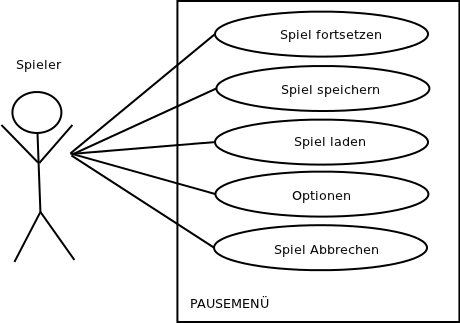
\includegraphics[width=90mm, height=58mm]
                  {kapitel/funktionen/Pausemenue.png}
	\end{center}
	\caption{Übersicht der Pausemenü-Funktionen}
	\label{fig:pausemenue_funktionen}
\end{figure}

\newpage

\paragraph{UseCase: Spiel pausieren}
\begin{center}
	\begin{tabular}{|r l|}
	  \hline
	  \textbf{Titel}: & Spiel pausieren\\
	  \textbf{Akteur}: & Spieler \\
	  \textbf{Fachlicher Auslöser}: & Spieler möchte Spiel unterbrechen \\
	  \textbf{Vorbedingungen}: & Spieler ist \textit{Ingame} \\
	  \hline
	  \textbf{Standardablauf}:
		& 1. Spieler: wählt Pausenmenü \\
		& 2. System: wechselt in den \textit{Menümodus} \\
		& 3. Spieler: wählt eine Pausefunktion aus \\
	  \textbf{Abbruch}:
                & 1.a Spieler: Spieler wählt \textit{Spiel fortsetzen} \\
		& 2.a System:  wechselt in den \textit{Ingamemodus} \\
	  \hline
	  \textbf{Nachbedingung}: & Spiel pausiert, System im Menümodus\\
	  \textbf{NF-Anf}.: & Reaktionszeit System $<$ 1 Sekunde \\
	  \textbf{Nutzungshäufigkeit}.: &  min. einmal pro Spiel \\
	  \hline
	\end{tabular}
\end{center}

\subsection{Speichern eines Spiels}
Das Spiel kann ausschließlich gespeichert werden, wenn der \gls{Spieler} sich im
Ingamemodus befindet. Dazu wählt er die entsprechende Taste zur Spielunterbrechung.
Darüber gelangt er dann in das Pausemenü. An dieser Stelle gibt es verschieden Auswahloptionen 
u.a. die das Spiel zu speichern. Geht der \gls{Spieler} in das Spiel speichern
Menü, kann er an dieser Stelle einen vorhandenen Spielstand aus einer Liste 
überschreiben oder einen neuen anlegen und so sein derzeitiges Spiel speichern. Ihm 
steht es jedoch frei auch einen Spielstand zu löschen oder ohne zu speichern das Menü 
zu verlassen.

\subsection{Laden eines Spiels}
Spiele können im CampusAdventure auf zwei Arten geladen werden. Zum einen direkt nach dem Starten
der Spieldatei. Der \gls{Spieler} erreicht dabei zunächst das Hauptmenü, in dem er neben anderen
Optionen, die des Spiel ladens hat. Das Spiel laden Menü selbst, ist vom Aufbau her gleich dem
Speichermenü. Es kann ein Spielstand aus der Liste gewählt werden und dieser wird entweder gelöscht,
geladen oder das Menü wird ohne jegliche Aktion wieder verlassen, was einen Abbruch darstellt. Die 
zweite Variante ist, dass während einer Spielunterbrechung ein anderer Spielstand geladen werden kann.
Hierzu befindet sich der \gls{Spieler},auf Grund der Spielunterbrechung, im Pausemenü. In diesem ist
dann das Spiel laden Menü integriert und nutzbar.
\newpage
\